\backmatter
\chapter{Appendix A: Permissions}

\thispagestyle{empty}
\begin{center}
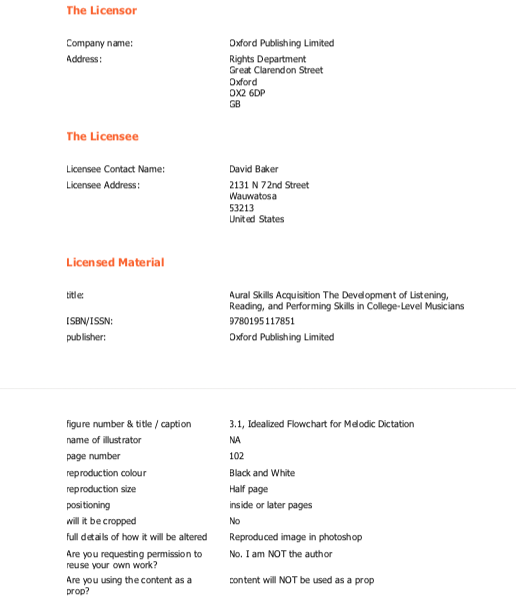
\includegraphics{karpinskipermission.png}
\end{center}

\chapter{Appendix B: Permissions}

\thispagestyle{empty}
\begin{center}
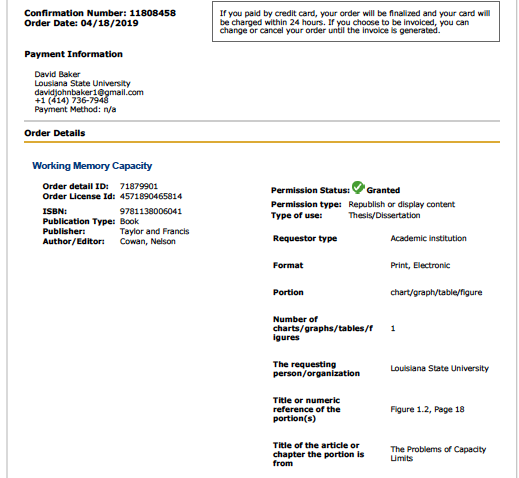
\includegraphics{cownpermission.png}
\end{center}

\chapter{Vita}

\doublespacing

David John Baker is a music researcher and educator passionate about questions at the intersection of music theory and music science.
His research looks to understand how the people learn melodies in order to improve pedagogical practices in aural skills education.
Initially trained as a conservatory musician-- studying under members of The Cleveland Orchestra at Baldwin Wallace University-- David has since completed an MSc in Music, Mind and Brain in London, England, and received his PhD in Music Theory at Louisiana State University where he completed his graduate minor in Cognitive and Brain Sciences.
Using his background in the humanities and training in psychological sciences, David builds testable models of how people hear music.
His overlapping quantitative skill set with the world of data science has also led him to both music industry projects and work in the non-profit/charity sector.
By combining knowledge at both the humanities and sciences, David believes that knowledge gained at this intersection will lead to world peace.






